 \documentclass{beamer}[10]

\usepackage{graphicx}
\usepackage{xcolor}
\usepackage{tabto}
%\usepackage{beamerthemesplit}
\usepackage{tikz}
\usepackage{cancel}
\usepackage{verbatim}
\usepackage{fancybox}
\usepackage{enumerate}
\usepackage{amsmath,amssymb,amsthm,textcomp,mathtools}
\usepackage[super]{nth}
\usepackage[amssymb]{SIunits}
\usepackage{booktabs}
\usepackage{cancel}
\usepackage{bm}
\usepackage[utf8]{inputenc}
\usepackage{tabularx}
\usepackage{ragged2e}
\newcolumntype{Y}{ >{\RaggedRight\arraybackslash}X}
\usetikzlibrary{arrows,shapes}
\newcommand\T{\rule{0pt}{2.6ex}}
\newcommand\B{\rule[-1.2ex]{0pt}{0pt}}
\definecolor{UUcrimson}{RGB}{204,0,0}
\mode<presentation>
{ \usetheme{default}
  \usecolortheme[named=UUcrimson]{structure}
  \useinnertheme{circles}
  \setbeamercovered{transparent}
  \setbeamertemplate{blocks}[rounded]
  \usefonttheme[onlymath]{serif}
  \setbeamertemplate{navigation symbols}{}
  \setbeamertemplate{footline}[page number]
  \setbeamertemplate{navigation symbols}{}
  \setbeamercolor{section in toc}{fg=black,bg=white}
  \setbeamercolor{alerted text}{fg=UUcrimson!80!gray}
  \setbeamercolor*{palette primary}{fg=white,bg=UUcrimson}
  \setbeamercolor*{palette secondary}{fg=UUcrimson!70!black,bg=gray!15!white}
  \setbeamercolor*{palette tertiary}{bg=UUcrimson!80!black,fg=gray!10!white}
  \setbeamercolor*{palette quaternary}{fg=UUcrimson,bg=gray!5!white}
  \setbeamercolor*{palette sidebar primary}{fg=UUcrimson!10!black}
  \setbeamercolor*{palette sidebar secondary}{fg=white}
  \setbeamercolor*{palette sidebar tertiary}{fg=UUcrimson!50!black}
  \setbeamercolor*{palette sidebar quaternary}{fg=gray!10!white}
  \setbeamercolor{titlelike}{parent=palette primary,fg=white}
  \setbeamercolor{frametitle}{bg=UUcrimson}
  \setbeamercolor{frametitle right}{bg=UUcrimson}
  \setbeamercolor*{separation line}{}
  \setbeamercolor*{fine separation line}{}
}

\usetikzlibrary{backgrounds}
\makeatletter
\tikzstyle{every picture}+=[remember picture]
\tikzset{%
  fancy quotes/.style={
    text width=\fq@width pt,
    align=justify,
    inner sep=1em,
    anchor=north west,
    minimum width=\linewidth,
    font=\itshape
  },
  fancy quotes width/.initial={.8\linewidth},
  fancy quotes marks/.style={
    scale=8,
    text=white,
    inner sep=0pt,
  },
  fancy quotes opening/.style={
    fancy quotes marks,
  },
  fancy quotes closing/.style={
    fancy quotes marks,
  },
  fancy quotes background/.style={
    show background rectangle,
    inner frame xsep=0pt,
    background rectangle/.style={
      fill=gray!25,
      rounded corners,
    },
  }
}
\newenvironment{fancyquotes}[1][]{%
\noindent
\tikzpicture[fancy quotes background]
\node[fancy quotes opening,anchor=north west] (fq@ul) at (0,0) {``};
\tikz@scan@one@point\pgfutil@firstofone(fq@ul.east)
\pgfmathsetmacro{\fq@width}{\linewidth - 2*\pgf@x}
\node[fancy quotes,#1] (fq@txt) at (fq@ul.north west) \bgroup}
{\egroup;
\node[overlay,fancy quotes closing,anchor=east] at (fq@txt.south east) {''};
\endtikzpicture}
\makeatother

\usepackage{scalerel}[2014/03/10]
\usepackage{stackengine}
\usepackage{empheq}
\newcommand*\widefbox[1]{\fbox{\hspace{0.5em}#1\hspace{0.5em}}}

\newcommand\reallywidetilde[1]{\ThisStyle{%
  \setbox0=\hbox{$\SavedStyle#1$}%
  \stackengine{-.1\LMpt}{$\SavedStyle#1$}{%
    \stretchto{\scaleto{\SavedStyle\mkern.2mu\sim}{.5467\wd0}}{.4\ht0}%
%    .2mu is the kern imbalance when clipping white space
%    .5467++++ is \ht/[kerned \wd] aspect ratio for \sim glyph
  }{O}{c}{F}{T}{S}%
}}
\usepackage{media9}

\logo{
\includegraphics[width=0.75cm]{logo.jpg}}
\author[Gibbs]{Dr. Jeremy A. Gibbs}
\institute{Department of Mechanical Engineering\\University of Utah}
\date{Fall 2016}
\title{LES of Turbulent Flows: Lecture 22}
\begin{document}

%----------------------------------------------------------------------------------------
%	TITLE & TOC SLIDES
%----------------------------------------------------------------------------------------

\begin{frame} 
  \titlepage
\end{frame}

%------------------------------------------------

\begin{frame}
\frametitle{Overview}
\tableofcontents
\end{frame}

%------------------------------------------------
\section{Surface/Wall Boundary Conditions} %
%------------------------------------------------
\begin{frame}{Surface/Wall Boundary Conditions}
\begin{itemize}
	\item In many flows of interest, a solid wall (or surface) is present in some way
	\item It can be very costly to fully resolve the effects of the wall and implement ``natural'' no-slip BCs
	\item Chapman (1979) performed the first analysis of grid-resolution requirements for LES of wall-bounded flows
\end{itemize}
\end{frame}
%------------------------------------------------
\begin{frame}{Surface/Wall Boundary Conditions}
We can divide the flow into 2 regions:
\begin{itemize}
	\item \textbf{Outer layer}:  viscosity isn't as important and grid resolution requirements are more or less (not including SGS model errors) independent of Re
	\item \textbf{Inner layer}:  near wall region where viscosity plays an important role
\end{itemize}
\end{frame}
%------------------------------------------------
\begin{frame}{Surface/Wall Boundary Conditions}
\textbf{Inner layer}:
\begin{itemize}
	\item Structures (``eddies'') in the inner-layer are approximately constant when non-dimensionalized with viscous length scales
	\item To resolve these motions we need grid spacing of
	\begin{align*}
		\Delta x^+ &\sim 100\quad (x^+ = x_i u_{\tau}/\nu)\\
		\Delta z^+ &\sim 20
	\end{align*}
	where $u_{\tau} = \sqrt{\cfrac{\tau_w}{\rho}}$ is the friction velocity
\end{itemize}
\end{frame}
%------------------------------------------------
\subsection{Requirements to Resolve the Wall}   %
%------------------------------------------------
\begin{frame}{Requirements to Resolve the Wall}
\begin{itemize}
	\item Using these $\Delta x^+$ and $\Delta z^+$ scales, we can show that
	$$N_x \times N_y \times N_z \propto \text{Re}_L^{1.8}$$
	where Re$_L$ is the integral scale Reynolds number -- that is the Reynolds number that is based on the integral length scale of turbulence
	\item The integral length scale is the characteristic length scale of the larger eddies in a turbulent flow
	\item In order to resolve the viscous sublayer (to enforce the use of the no-slip condition), the number of required grid points scales as Re$_L^{1.8}$
	\item Conversely, Chapman (1979) showed that the number of grid points required to resolve the outer layer scales as Re$_L^{0.4}$
\end{itemize}
\end{frame}
%------------------------------------------------
\begin{frame}{Requirements to Resolve the Wall}
\begin{itemize}
	\item For a BL with Re$_L=10^6$ (moderate-low Re), \textbf{99\% of our grid points} must be in the near wall region
	\item This region is only \textbf{10\% of the entire boundary layer! }
\end{itemize}
\begin{figure}
	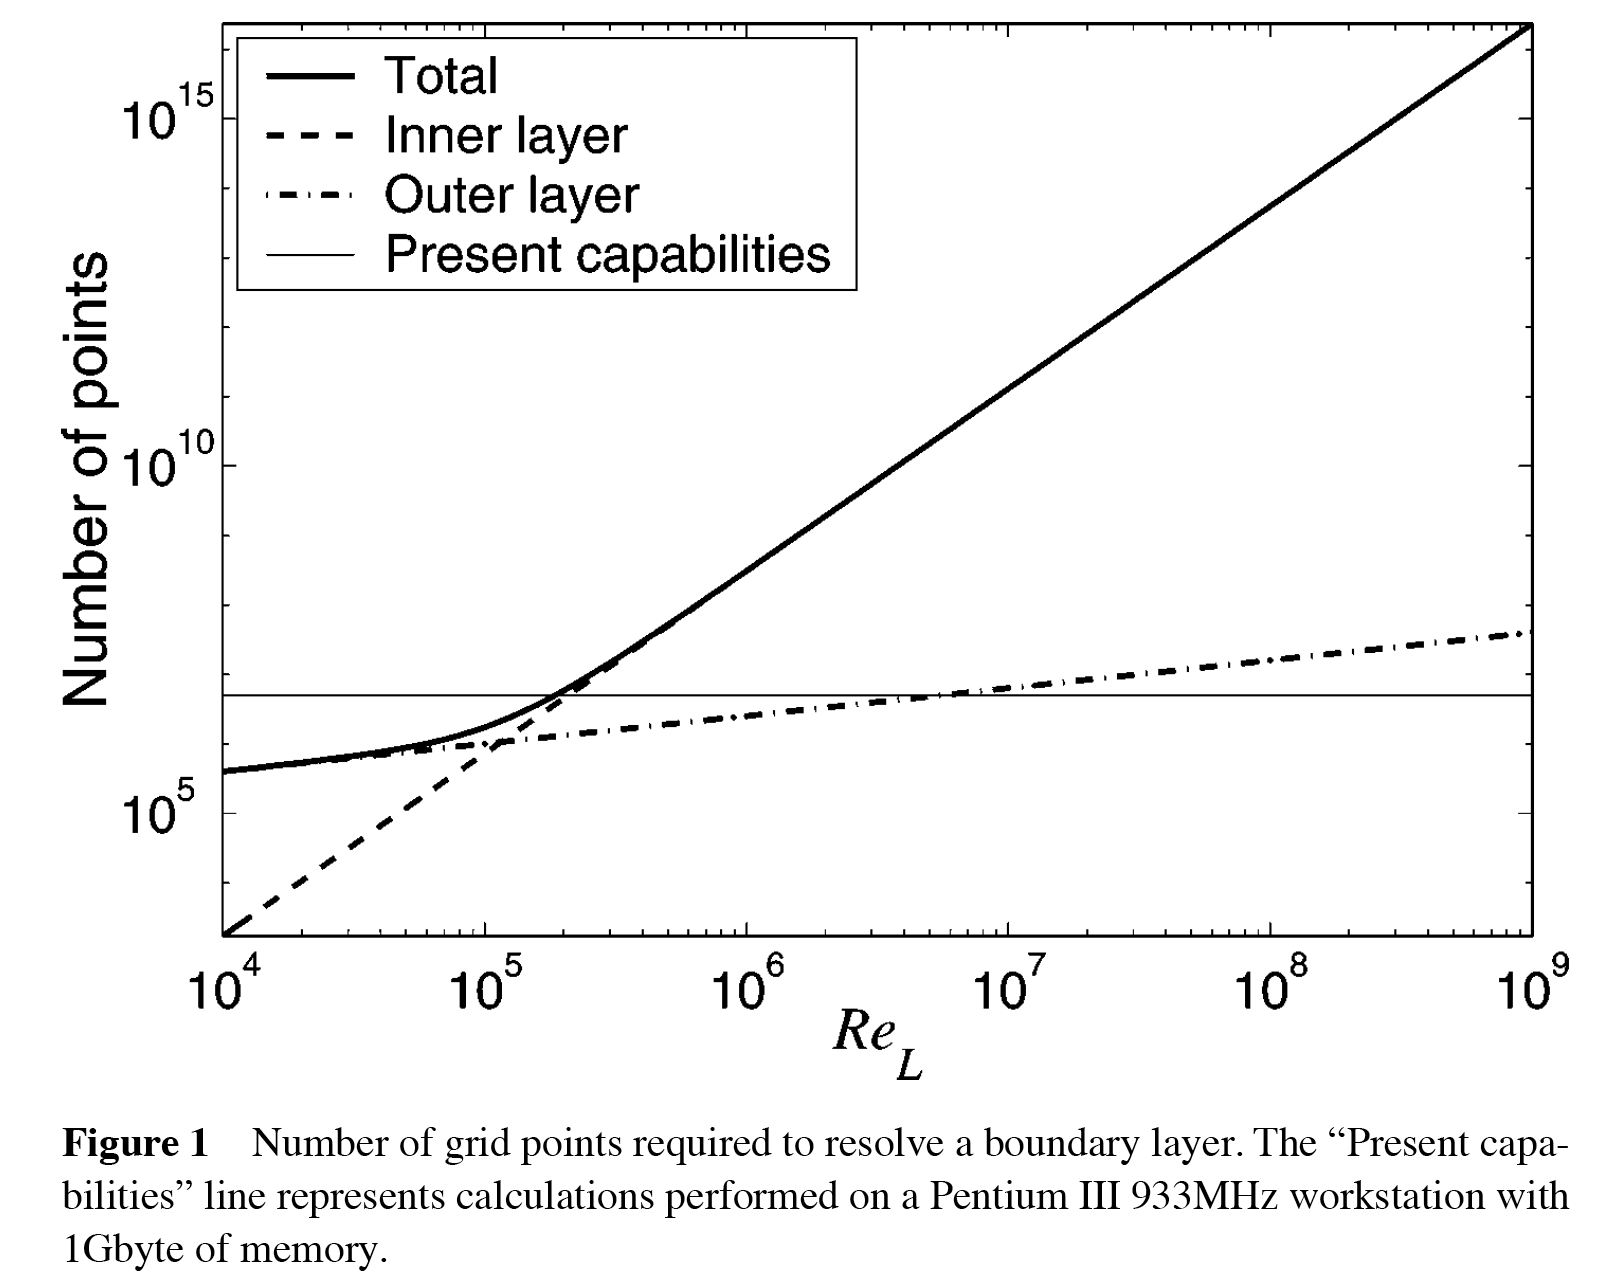
\includegraphics[width=0.75\textwidth]{sbc1}
\end{figure}

\end{frame}
%------------------------------------------------
\subsection{Approximate Wall-Boundary Conditions} %
%------------------------------------------------
\begin{frame}{Approximate Wall-Boundary Conditions}
\begin{itemize}
	\item How do we handle this problem for high-Re boundary layers?
	\item Answer: with \textbf{approximate wall-boundary conditions}
	\begin{itemize}
		\item We pick our first grid-point to be sufficiently far from the wall so it lies in the outer layer
		\item This has the \textbf{potential to make our simulations only weakly dependent on Re and grid resolution} (if we don’t consider model errors!)
		\item The \textbf{goal is to create a model} that calculates the \textbf{wall shear stress as a function of the resolved velocity} at the lowest grid level
		\item \textbf{All of the dynamics of the inner layer} must be accounted for with the wall model
	\end{itemize}
\end{itemize}

\end{frame}
%------------------------------------------------
\begin{frame}{Approximate Wall-Boundary Conditions}
\begin{figure}
	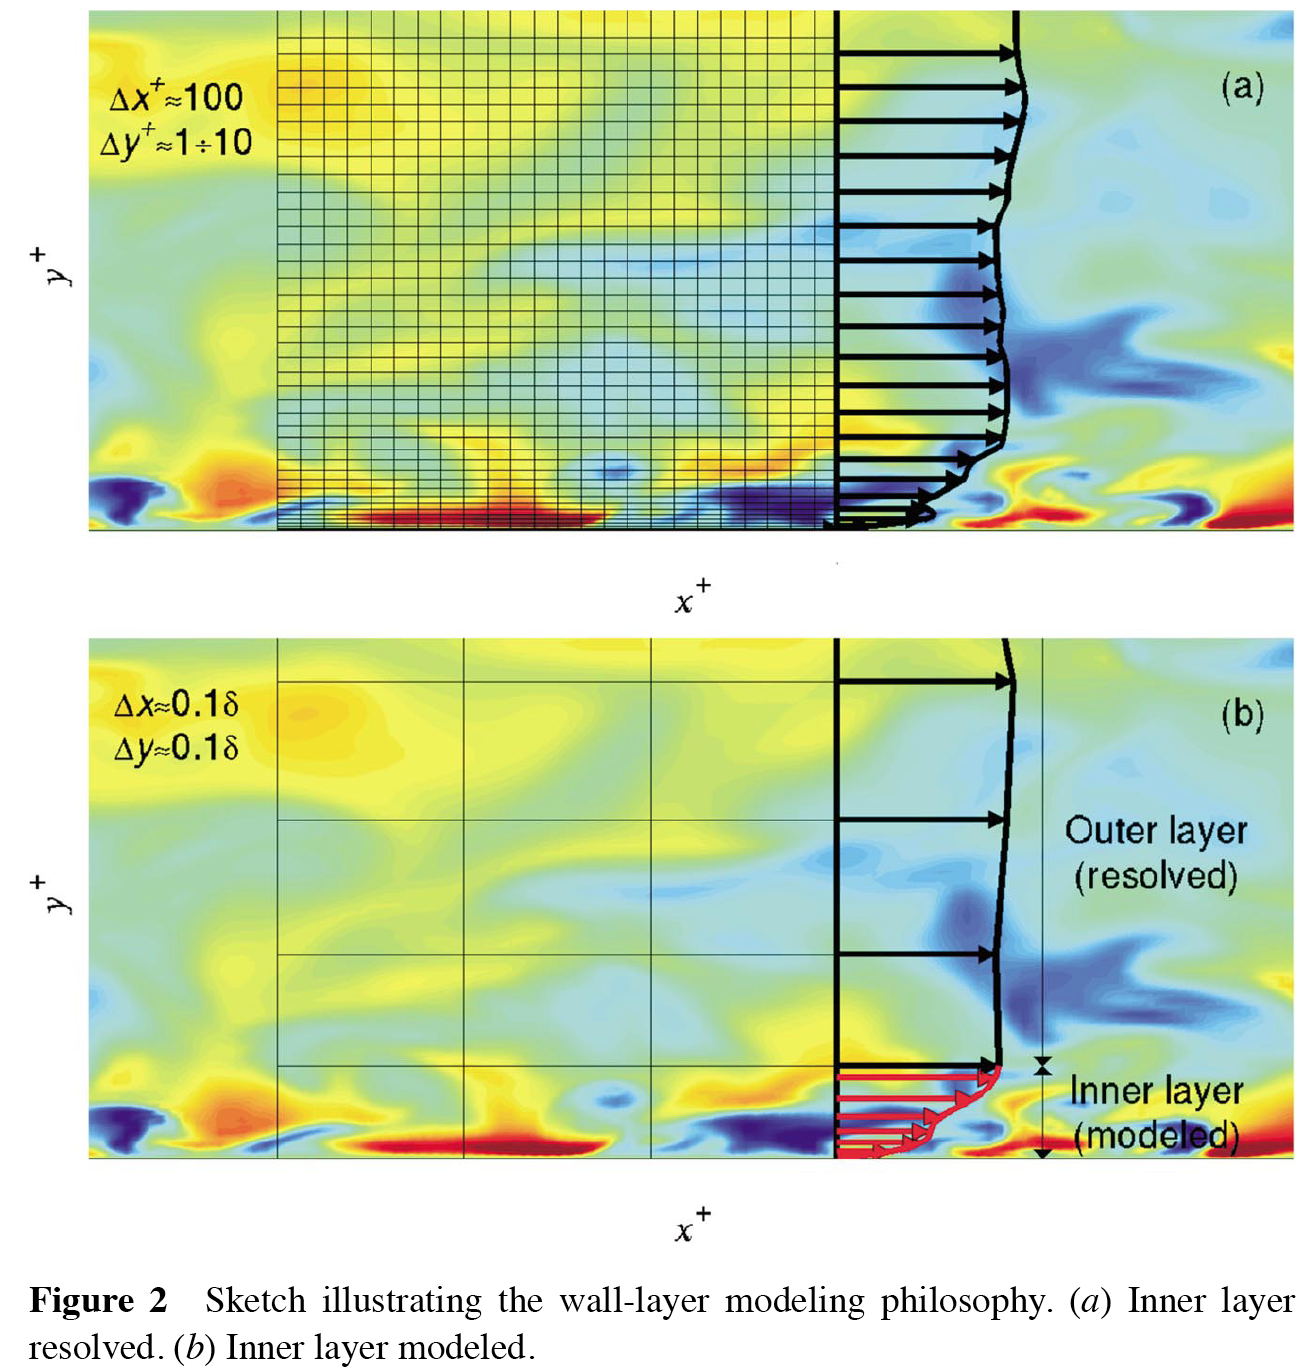
\includegraphics[width=0.65\textwidth]{sbc2}
\end{figure}
\centering From Piomelli and Balaras (2002)
\end{frame}
%------------------------------------------------
\begin{frame}{Approximate Wall-Boundary Conditions}
\textbf{Typical high-Re wall models}
\begin{itemize}
	\item Many wall models use RANS-like approximations
	\item In high-Re BLs, the most common models are \nth{0}-order RANS (\textit{i.e.} similarity theory)
	\item $\tilde{u}_i$ and $\tau_w$ are assumed to be related by the well known log-law
	\item For a rough-wall:
	$$U(z) = \frac{u_\tau}{\kappa} \left[\ln \left(\frac{z}{z_o}\right) - \Psi_M\left(\frac{z}{L}\right)\right]$$
	where $U(z)$ is the mean velocity, $u_\tau = \sqrt{-\tau_w}$ is friction velocity, $z$ is the height of the first model level, $z_o$ is the surface roughness, and $\Psi_M$ is the stability correction function
\end{itemize}

\end{frame}
%------------------------------------------------
\begin{frame}{Approximate Wall-Boundary Conditions}
\textbf{Typical high-Re wall models}
\begin{itemize}
	\item Schumann (1975) introduced the \newline of this class of models where:
	$$\tau_{i3,w}(x,y,t) = \langle \tau_w \rangle \frac{\tilde{u}_i(\vec{x},t)}{U(z)} \quad \text{for $i=1,2 (x,y)$} $$
	\item $\langle \tau_w \rangle$ was calculated from the mean pressure gradient
\end{itemize}

\end{frame}
%------------------------------------------------
\begin{frame}{Approximate Wall-Boundary Conditions}
\textbf{Typical high-Re wall models}
\begin{itemize}
	\item Gr{\"o}tzbach (1987) modified this by using the log-law to calculate the average shear stress resulting in the flowing model
	$$\tau_{i3,w}(x,y,t) = - \left[\frac{U(z)\kappa}{\ln(z/z_o) - \Psi_M}\right] \left[\frac{\tilde{u}_i(\vec{x},t) \kappa}{\ln(z/z_o) - \Psi_M}\right]$$
	\item This model has the advantage over Schumann's because it allows the total mass flux to change in time during a simulation
	\item Both models assume that $\tau_w \sim \tilde{u}_i$
\end{itemize}

\end{frame}
%------------------------------------------------
\subsection{Accounting for Flow Average Flow Structures} %
%------------------------------------------------
\begin{frame}{Accounting for Flow Average Flow Structures}
\begin{itemize}
	\item Piomelli et al. (1989) altered the models of Schumann and Gr{\"o}tzbach (SG) in an attempt to account for the structure of the flow field
	\item Experimental and numerical studies have demonstrated that coherent structures exist in the BL and that they are inclined at oblique angles to the wall (\textit{e.g.} Brown and Thomas 1977)
\end{itemize}
\vspace{-10pt}
\begin{figure}
	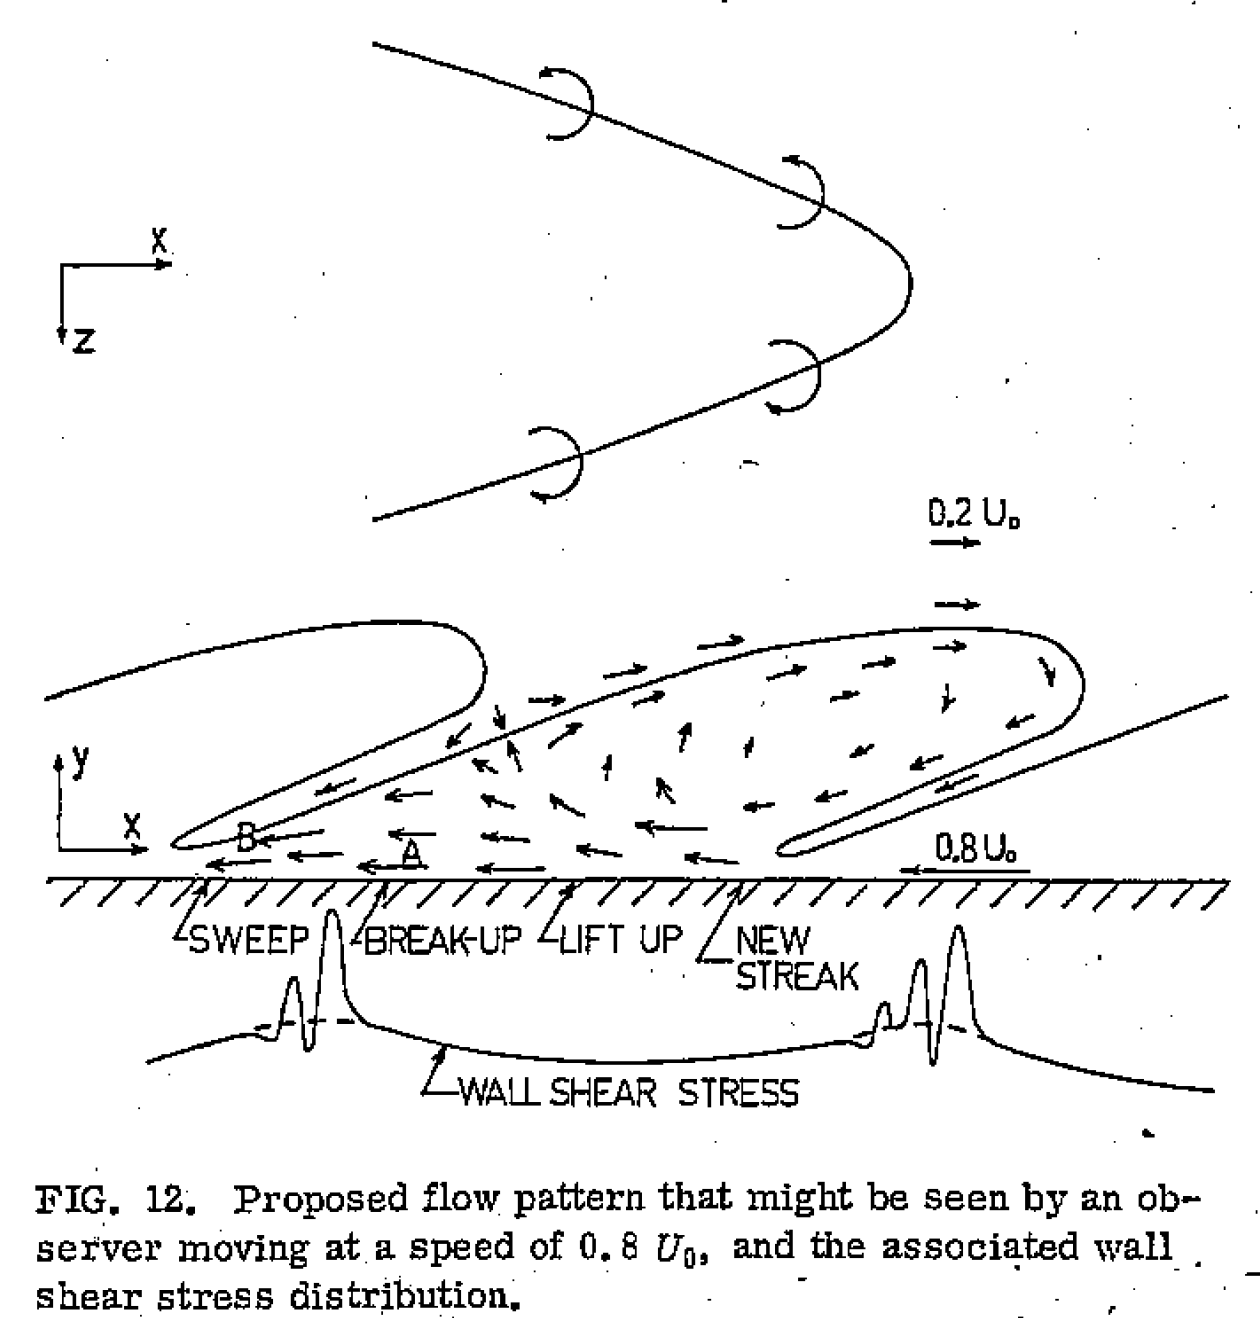
\includegraphics[width=0.47\textwidth]{sbc3}
\end{figure}
\end{frame}
%------------------------------------------------
\begin{frame}{Accounting for Flow Average Flow Structures}
\begin{itemize}
	\item The inclination of these structures can be measured by looking at the correlation between shear stress and velocity in a BL
	\item With the average inclination given by the lag to max correlation with height
\end{itemize}
\begin{figure}
	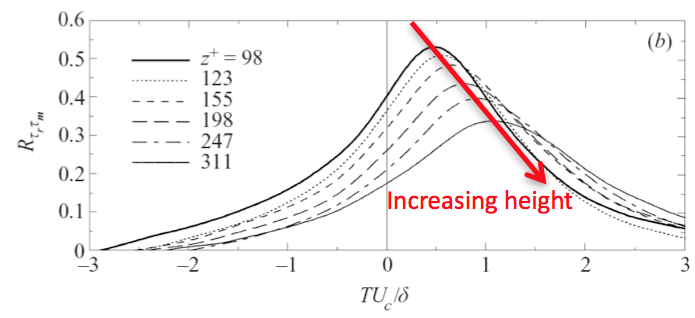
\includegraphics[width=0.8\textwidth]{sbc4}
\end{figure}
\centering From Marusic et al (2001)
\end{frame}
%------------------------------------------------
\begin{frame}{Accounting for Flow Average Flow Structures}
\begin{itemize}
	\item Another example taken from an idealized LLJ simulation
\end{itemize}
\begin{figure}
	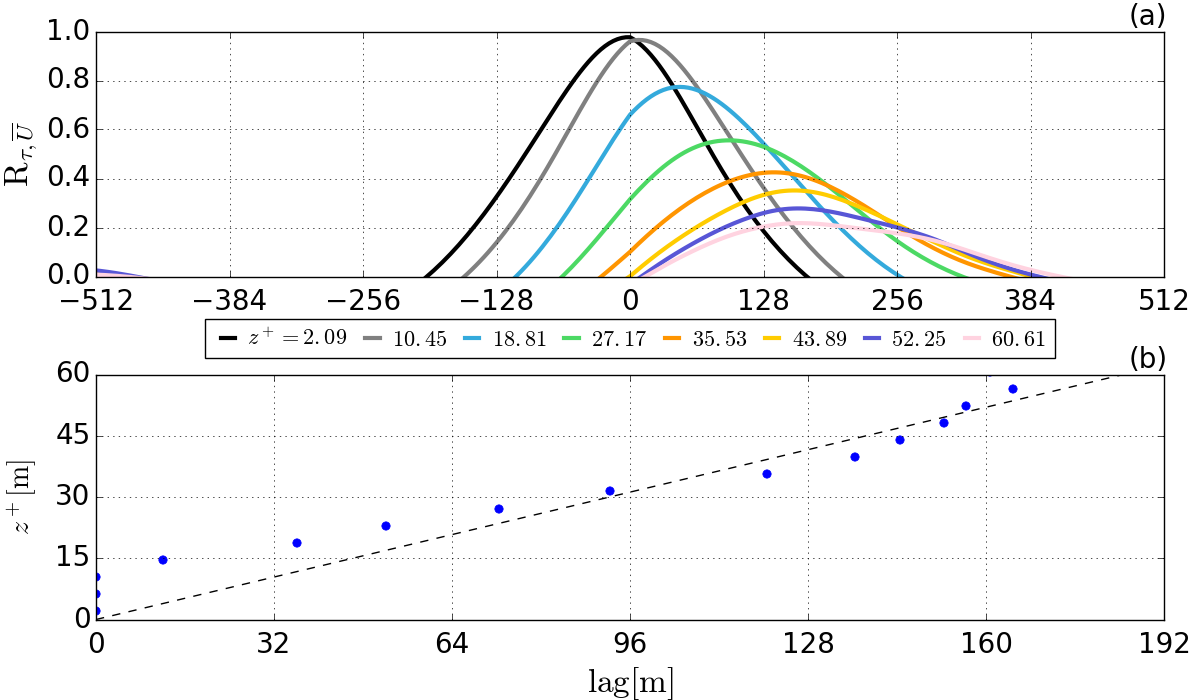
\includegraphics[width=1\textwidth]{sbc5}
\end{figure}
\end{frame}
%------------------------------------------------
\begin{frame}{Accounting for Flow Average Flow Structures}
\begin{itemize}
	\item Piomelli et al. (1989) took this into account by shifting the SG model downstream
	$$\tau_{i3,w}(x,y,t) = \langle \tau_w \rangle \frac{\tilde{u}_i(x + \delta_d,y,z,t)}{U(Z)}$$
	where $\delta = z\;\cot({\gamma})$ is the displacement and $\gamma \approx 13^\circ$ for high-Re flows
\end{itemize}
\end{frame}
%------------------------------------------------
\begin{frame}{Approximate Wall-Boundary Conditions}
\begin{columns}[T]
    \begin{column}{.55\textwidth}
    \begin{minipage}[c][.8\textheight][c]{\linewidth}
    \textbf{a priori analysis}
    \begin{itemize}
	\item Analysis of hotwire data from Marusic et al (2001)
	\item Found low correlation between SG model and measured data
	\item Figures show: time series of SG model vs. data (a), 2pt correlations from the SGS model (b) and shear stress spectra from SG model (c) from Marusic et al (2001)
\end{itemize}
      \end{minipage}
    \end{column}
    \begin{column}{.55\textwidth}
      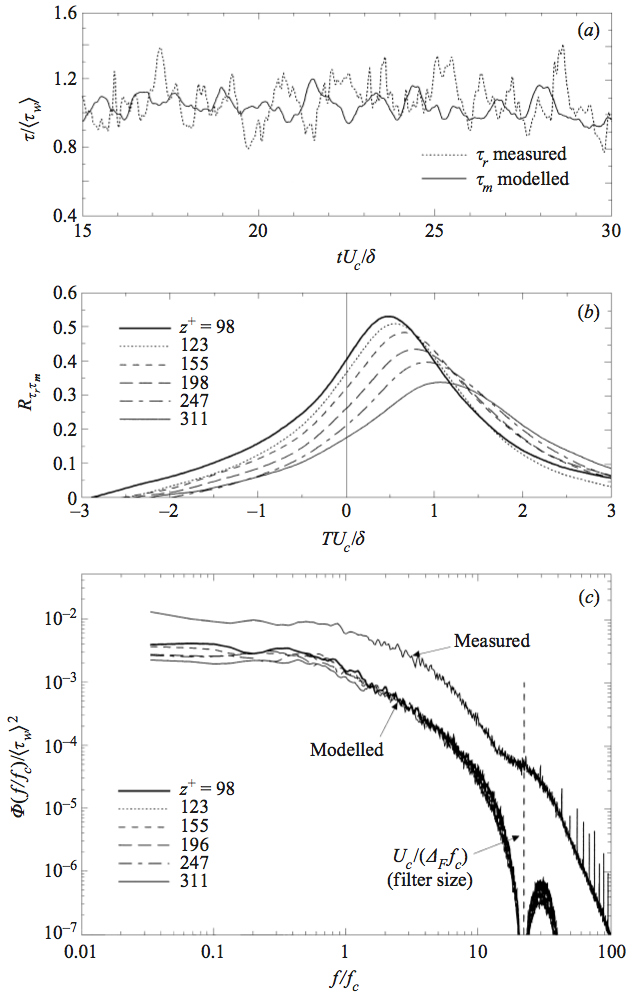
\includegraphics[width=0.87\textwidth]{sbc6}
    \end{column}
  \end{columns}
\end{frame}
%------------------------------------------------
\begin{frame}{Approximate Wall-Boundary Conditions}
\textbf{a priori analysis}
\begin{itemize}
	\item Based on their analysis, Marusic et al (2001) proposed a new model
	$$\tau_{i3,w}(x,y,t) = \langle \tau_w \rangle - \alpha u_\tau \left[ \tilde{u}_i (x + \Delta,y,z,t) - \langle \tilde{u}_i (x+\Delta,y,z,t)\rangle \right]$$
	\item Basic motivation: low frequency filtered velocity spectra will collapse under outer-flow scaling and that the filtered shear stress spectra should follow the filtered velocity spectra
	\item Based on this, $\alpha$ should be a constant under a variety of conditions
\end{itemize}
\end{frame}
%------------------------------------------------
\begin{frame}{Approximate Wall-Boundary Conditions}
\textbf{a priori analysis}
\begin{itemize}
	\item Following Stoll and Port\'{e}-Agel (2006) we can compare
this to the SG model
	\begin{align*}
	\tau_{i3,w}(x,y,t) &= \langle \tau_w \rangle \frac{\tilde{u}_i (x + \Delta,y,z,t)}{U_i(z)}\\
	&= \langle \tau_w \rangle + \frac{\langle \tau_w \rangle}{U_i(z)} \left[ \tilde{u}_i(x+\Delta,y,z,t) - U_i(z)\right]\\
	&= \langle \tau_w \rangle - \alpha_{eq} u_\tau \left[ \tilde{u}_i(x+\Delta,y,z,t) - U_i(z)\right]
	\end{align*}
	where
	$$\alpha_{eq} = \frac{\langle \tau_w \rangle}{u_\tau U_i(z)} = \frac{\kappa}{\ln(z/z_o)}$$
\end{itemize}
\end{frame}
%------------------------------------------------
\begin{frame}{Approximate Wall-Boundary Conditions}
\textbf{a priori analysis}
\begin{figure}
      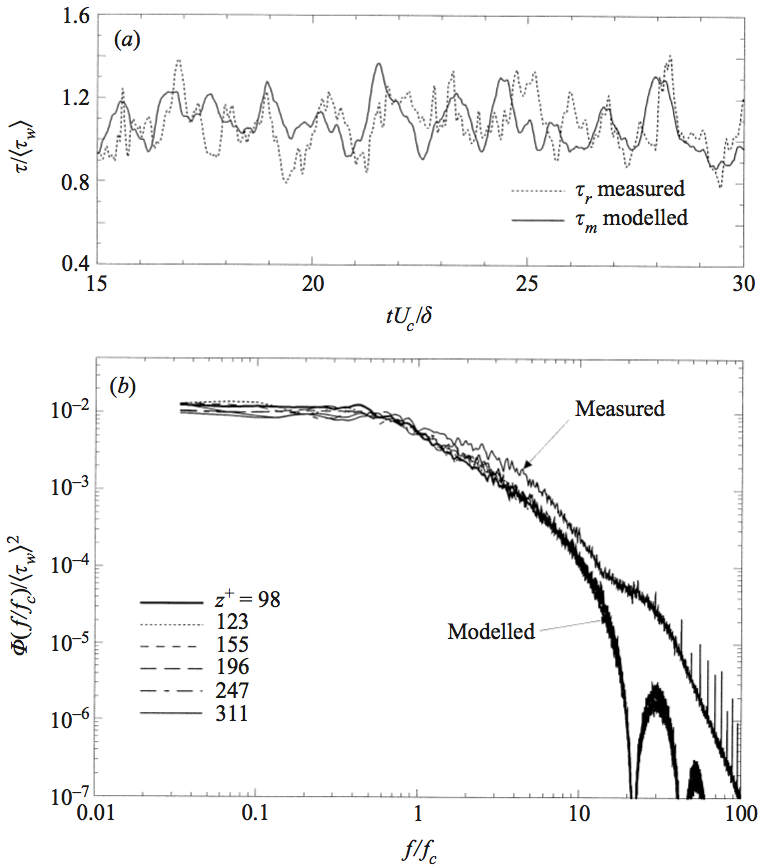
\includegraphics[width=0.63\textwidth]{sbc7}
\end{figure}
\end{frame}
%------------------------------------------------
\section{Local and Higher-order RANS Approximations} %
%------------------------------------------------
\begin{frame}{Local and Higher-order RANS Approximations}
\textbf{The local log-law for ABL flows}
\begin{itemize}
	\item In the ABL or general flows where no directions of homogeneity exist for determining
 $\langle \tau_w \rangle$, the log-law is often used directly to calculate the local shear stress by
	$$\tau_{i3,w} (x,y,t) = - \left[ \frac{\tilde{u}_r (\vec{x},t)\kappa}{\ln(z/z_o) - \Psi_M}\right]^2 \left[ \frac{\tilde{u}_i (\vec{x},t)}{\tilde{u}_r (\vec{x},t)}\right]$$
	where
	$$\tilde{u}_r = \sqrt{\tilde{u}_x^2 + \tilde{u}_y^2}$$
	\item The formulation assumes $\tau_w \sim \tilde{u}_i^2$ and does not preserve $\langle \tau_w \rangle$
\end{itemize}
\end{frame}
%------------------------------------------------
\begin{frame}{Local and Higher-order RANS Approximations}
\textbf{2-layer models (higher-order RANS):}
\begin{itemize}
	\item Balaras et al., (AIAA, 1996) used a higher order RANS closure based on the thin-BL equations
	$$\frac{\partial \tilde{u}_i}{\partial t} + \frac{\partial}{\partial x_i}(\tilde{u}_n \tilde{u}_i) = -\frac{\tilde{p}}{\partial x_i} + \frac{\partial}{\partial x_n}\left[ (\nu + \nu_T)\frac{\partial \tilde{u}_i}{\partial x_n}\right]$$
	where $i=1,2$, $u_n$ is the wall normal component found from continuity and $\nu_T$ is an eddy-viscosity parameterized with an algebraic model. The equations are solved to the wall.
\end{itemize}
\end{frame}
%------------------------------------------------
\begin{frame}{Local and Higher-order RANS Approximations}
\textbf{2-layer models (higher-order RANS):}
\begin{figure}
      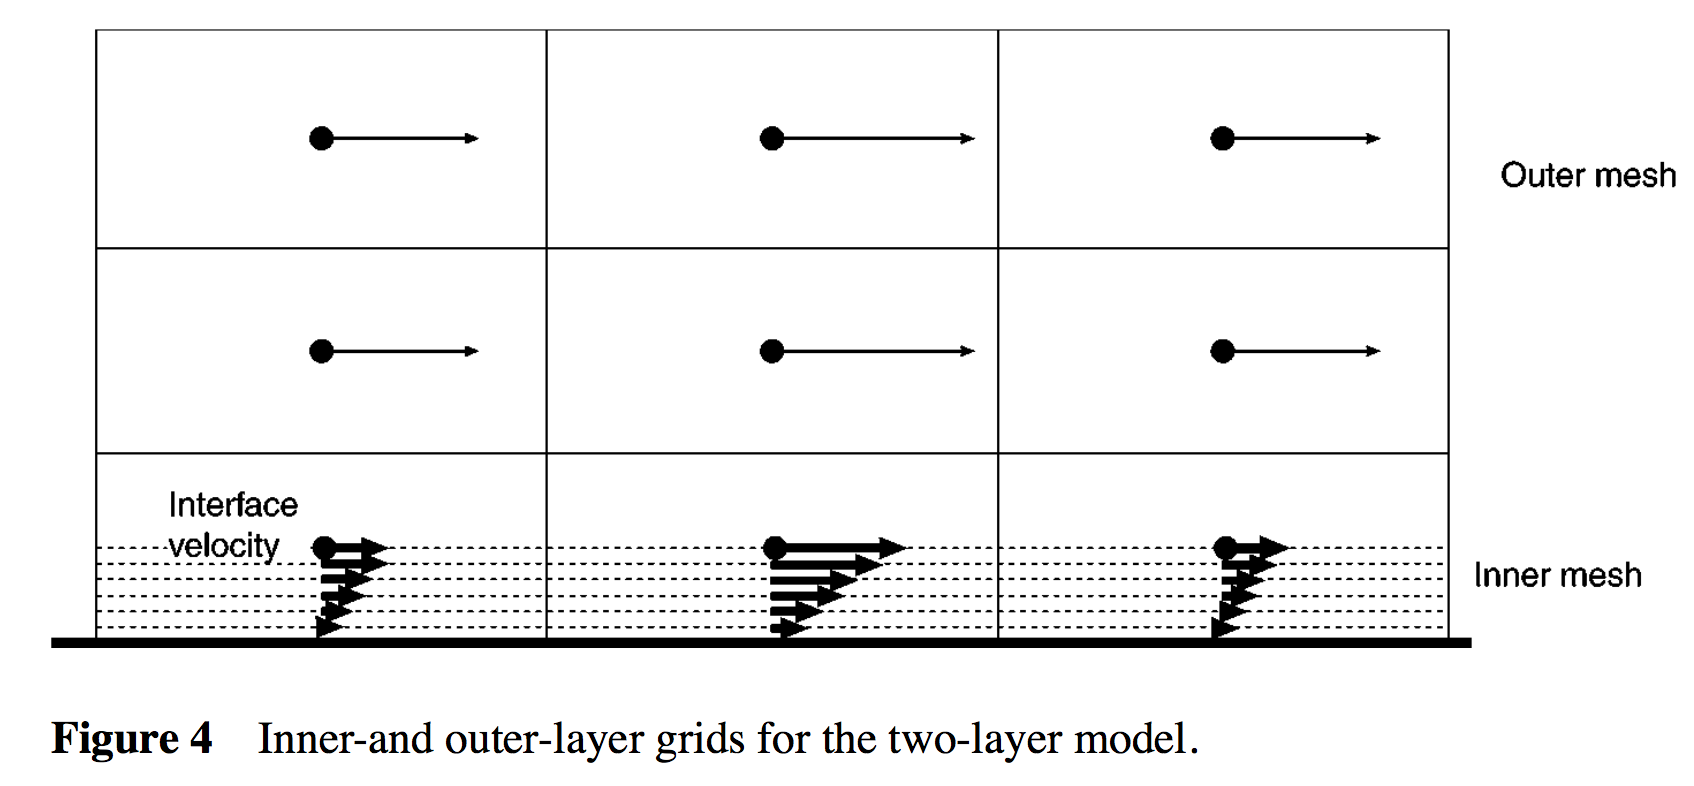
\includegraphics[width=\textwidth]{sbc8}
\end{figure}
\centering From Piomelli and Balaras (2002)
\end{frame}
%------------------------------------------------
\begin{frame}{Even more variations}
\textbf{The filtered local log-law for ABL flows:}
\begin{itemize}
	\item Bou-Zeid et al. proposed to use the filtered velocity to find the surface stress
	$$\tau_{i3,w}(x,y,t) = \left[ \frac{\bar{\tilde{u}}_i (x+\Delta,y,z,t)\kappa}{\log(z/z_o)}\right]^2 \frac{\tilde{u}_i (x+\Delta,y,z,t)}{\bar{\tilde{u}}_i (x+\Delta,y,z,t)}$$ 
	\item Poimelli et al. (1989) -- and others -- suggested using the wall normal velocity
	$$\tau_{i3,w}(x,y,t) = \langle \tau_w \rangle - C\langle \tau_w \rangle^{1/2} \tilde{w}(x+\Delta,y,t)$$
	\item  Hultmark et al. (2013) suggested using velocity variance scaling to develop a local correction for the problem that the instantaneous log-law above won't preserve the mean shear stress value
\end{itemize}
\end{frame}
%------------------------------------------------


\end{document}

